\chapter{GraphQL}
\section{Typ-System}

Das GraphQL-Typ-System wird zur Definition eines Schemas verwendet.
Ein Schema beschreibt einen GraphQL-Service und besteht aus den abrufbaren Ressourcen, ihren Relationen zueinander und ihren Interaktionsmöglichkeiten.


Eine eingehende Anfrage wird durch die im Schema definierte Datenstruktur validiert.
Wenn die in der Anfrage enthaltene Query durch das Typ-System erfolgreich validiert wurde, wird die beinhaltete Operation an die Implementierung weitergeleitet.
Dafür zerlegt GraphQL die übergebene Query und gibt sie an den jeweiligen Resolver weiter. Diese Resolver interagieren mit der Geschäftslogik und füllen die angeforderten Felder mit Daten.
Die kumulierten Ergebnisse werden als Antwort an den Client zurückgeschickt. 
\cite[S. 57-58]{kress2020graphql}
\cite[Abs. Schemadefinition]{graphqlOnline}


\section{Schema-Definitions-Sprache SDL}
Da GraphQL laut Spezifikation in jeder beliebigen Sprache implementierbar sein soll, wird eine sprachunabhängige Basis für die Definition des GraphQL-Graphen benötigt.
Die Grundlage dafür stellt die in der Spezifikation definierte Beschreibungssprache (\textit{SDL}). 
In GraphQL existieren folgende Typ-Definitionen: \textit{Skalar, Interface, Object, Input Object, Enum} und \textit{Union}.
Diese bilden das Rückgrat des Schemas.
Diese Typen werden in den nachfolgenden Abschnitten genauer behandelt.

% \subsection{Skalare}
\myparagraph{Skalare}

Ein Datentyp, der nicht mehr weiter vereinfachbar ist, wird wie in anderen Programmiersprachen Skalar-Typ genannt.
Skalar-Typen repräsentieren die Blätter, also die primitiven Werte des GraphQL-Typ-Systems \cite[S. 60]{kress2020graphql}.
GraphQL-Antworten entsprechen der Form eines hierarchisch aufgebauten Baumes.
\newline


Grundsätzlich bestehen die Blätter dieses Baumes aus GraphQL-Skalar-Typen (es ist zudem auch möglich, dass die Blätter aus \textit{Null-Werten} oder \textit{Enum-Typen} bestehen).
\cite[Abs. ScalarTypeDefinition]{graphqlOnline}
GraphQL beinhaltet folgende vordefinierten Skalar-Typen:
\begin{enumerate}
    \item Boolean
    \item Float
    \item Int
    \item String
    \item ID
\end{enumerate}

\begin{JsCode}
    id: Int!
    title: String
\end{JsCode}

Im oben angeführten Codebeispiel werden die Felder \textit{id} und \textit{title} definiert.
Der Name eines Feldes im umgebenden Typ muss dabei eindeutig sein.
Die Deklaration erfolgt mit dem Namen als auch dem Typ des Feldes, welche mit einem Doppelpunkt getrennt sind.
Das Feld \textit{id} wird dabei mit einem Rufzeichen (!) als \textit{not null} deklariert.

In den meisten sprachspezifischen Implementierungen ist es möglich, eigene Skalar-Typen zu definieren. Diese werden verwendet, um beispielsweise verschiedene Datumsformate darzustellen.

% \subsection{Enum}
\myparagraph{Enum}

Enum-Typen stellen wie Skalare die Blätter des Typ-Baums dar.
Ein Enum-Feld hält ein spezifisches Element aus einer Menge von möglichen Werten
\cite[Abs. 3.9]{graphqlOnline}
\cite[S. 60-61]{kress2020graphql}.

\begin{JsCode}
enum Category {
    Fantasy
    Adventure
    Mystery
    Thriller
    Romance
}
\end{JsCode}

In diesem Beispiel wurde ein Enum \textit{Category} definiert.
Es gilt zu beachten, dass dieser Typ mit dem Schlüsselwort \textit{enum} definiert werden muss.

% \subsection{Objekt}
\myparagraph{Objekt}
Wie bereits erwähnt bestehen die Blätter des Baumes in GraphQL aus den Skalar-Typen.
Die Knoten wiederum werden von Objekt-Typen definiert.
Diese Objekte halten eine Liste von Feldern die einen bestimmten Wert lieferen.
Jedes Feld kann entweder ein Skalar, ein Enum, ein Objekt oder ein Interface sein.
Laut Spezifikation, sollten Objekte als eine Menge von geordneten Schlüssel-Wert-Paaren serialisiert werden.
Wobei der Name des Feldes der Schlüssel ist und das Ergebnis der Evaluierung des jeweiligen Feldes den Wert abbildet.
Um einen Objekt-Typ zu definieren muss das Schlüsselwort \textit{type} verwendet werden
\cite[Abs. 3.6]{graphqlOnline}.

\begin{JsCode}
type Book {
    id: Int!
    title: String
    authors: [Author]
}
    
type Author {
    id: Int!
    firstName: String
    lastName: String
    books: [Book]
}
\end{JsCode}

Im oben angeführten Schemaausschnitt werden die beiden Objekte \textit{Author} und \textit{Book} definiert.
Um einen Objekttypen zu definieren wird das Schlüsselwort \textit{type} verwendet.

Das Objekt Book wird dabei mit den Feldern \textit{id, title} und \textit{authors} definiert.
Das Objekt Author erhält die Felder \textit{id, firstName, lastName} und \textit{books}.

Die Felder \textit{id, title, firstName} und \textit{lastName} sind dabei skalare Felder und bilden dabei Blätter des Baumes.
Da zwischen den Objekten Author und Book eine n:m Beziehung besteht, halten beide Objekte eine Liste des jeweils anderen Objekt-Typs.
Listen werden in der SDL wie im obigen Beispiel ersichtlich mit eckigen Klammern definiert.

% \subsection{Interface}
\myparagraph{Interface}
Interfaces sind abstrakte Typen welche eine Liste an Feldern definieren.
GraphQL-Interfaces repräsentieren eine Liste von Felder und deren Argumente.
Objekte und Interfaces können ein Interface implementieren, dazu muss der Typ, welcher das Interface definieren will, alle Felder des zu implementierenden Interfaces definieren.
\newline
\cite[Abs. 3.7]{graphqlOnline}
Felder eines Interfaces sind an dieselben Regeln wie ein Objekt gebunden.
Der Typ eines Feldes kann entweder ein Skalar, Enum, Interface oder Union sein.
Zudem ist es möglich, dass ein Typ mehrere Interfaces implementiert.
\cite[S.65-66]{kress2020graphql}
\newline


Im folgenden Codebeispiel wird die Definition eines Interfaces veranschaulicht:

\begin{JsCode}
interface Person {
    firstName: String
    lastName: String
}

type Author implements Person {
    id: Int!
    firstName: String
    lastName: String
    books: [Book]
}
\end{JsCode}

Jedes Interface benötigt eine spezifische Implementierung, im angeführen Beispiel implementiert \textit{Author} das Interface \textit{Person}.
Author muss dabei alle Felder von \textit{Person} zur Verfügung stellen.

% \subsection{Input-Objekt}
\myparagraph{Input-Objekt}
Ein Input-Objekt ist ein spezieller Objekt-Typ. Ein Input-Objekt hält genauso wie ein Objekt-Typ skalare Felder, Enumerationen oder Referenzen.
Diese referenzierten Objekt-Typen müssen aber ebenso Input-Objekte sein.
Eine Mischung der Objekt-Typen ist laut Spezifikation nicht erlaubt.
Ein Input-Objekt unterscheidet sich zu einem Objekt-Typ nur durch das Schlüsselwort \textit{input} anstatt von \textit{type}.
Weiters können die Felder eines Input-Objekts keine Argumente beinhalten.
\newline


Im folgenden Beispiel wird ein Input-Objekt für ein Buch realisert:
\begin{JsCode}
input AuthorCreateInput {
  firstName: String
  lastName: String
  books: [Int!]
}
\end{JsCode}

% \subsection{Fragmentierung}\label{sec:Bezeichnung}
\myparagraph{Fragementierung}

Fragmente helfen dabei den Text von Abfragen zu reduzieren indem sie oft gebrauchte Abfragen von Feldern kapseln.
Weiters können Fragmente nur für Objekt-Typen, Interfaces und Union-Typen definiert werden.
Fragmente müssen dabei den Objekt-Typen für den sie gelten mit dem Schlüsselwort  \textit{on} angeben.
Inline-Fragmente müssen nicht mit dem Schlüsselwort \textit{fragment} definiert werden.
Sie können mit dem Spread-Operator direkt in der Abfrage definiert werden \cite[Abs. 2.8 -  2.8.1]{graphqlOnline}.
Fragmente liefern nur dann Daten zurück wenn der Objekt-Typ der sie anfordert auch wirklich dem Typen des Fragments entspricht.

Im folgenden Beispiel wird ein Fragment für den Objekt-Typ Author definiert, weiters wird die Verwendung in einer Query veranschaulicht:
\begin{JsCode}
fragment authorFragment on Author {
    firstName
    lastName
}

\end{JsCode}


Im nachfolgenden Beispiel wird die Nutzung eines Inline-Fragments in einer Query veranschaulicht:
\begin{JsCode}
query{
    books{
        title
        on Author{
            firstName
            lastName
        }
    }
}
\end{JsCode}

% \subsection{Union}
\myparagraph{Union}
Union-Typen fügen mehrere Objekte zu einer Gruppe zusammen.
Diese Typen sind sehr nützlich, wenn beispielsweise eine Query zwei unterschiedliche Objekt-Typen zurückgeben kann, diese aber nicht diesselben Felder besitzen.
In dieser Query können dann mithilfe von Inline-Fragmenten (siehe \ref{sec:Bezeichnung}) die spezifischen Felder abgefragt werden.

\begin{JsCode}
union SearchResult = Author | Buch
\end{JsCode}

% \subsection{Direktive}
\myparagraph{Direktive}
Direktiven bieten die Möglichkeit die Struktur, des durch eine Query angefragtes Ergebnis zu beeinflussen.
Mittels einer Annotation direkt an einem Feld oder einer Objekt-Relation
Mit Direktiven ist es möglich mittels Annotationen, direkt an einem Feld oder einem Objekt-Typen, dasselbige entsprechend einer Eingabe zu beeinflussen.
GraphQL bietet dafür standardmäßig zwei Arten von Strukturmanipulationen: \textit{@include} und \textit{@skip}, es ist aber auch möglich serverseitig zusätzliche Direktiven zu implementieren.
Mittels diesen Direktiven lassen sich Objekt-Typen oder Felder inkludieren oder überspringen.
Für die auszuwertende Direktive muss dabei in der Query ein \textit{Boolean} mitübergeben werden.

Im folgenden Beispiel wird eine Direktive gezeigt welche nach Bedarf das Feld \textit{id} ignoriert.

\begin{JsCode}
query {
    authors($withoutId: Boolean = false){
        id @include(if: $withoutId)
        firstName
        lastName
    }
}
\end{JsCode}


\section{Schema}
Im Schema welches mittels der \textit{SDL} definiert wird, werden alle Objekt-Typen des GraphQL-Services definiert.
Durch das Schema werden die verwalteten Entitäten durch Objekt-Typen definiert.
Weiters werden auch die vom GraphQL zur Verfügung gestellten Interfaces, Unions, Fragments, Direktiven, Enums und Input-Typen definiert.
Wenn man die im Schema definierten Objekt-Typen als Baumstruktur betrachtet so sind die referenzierten Objekt-Typen Verzweigungen des Baumes.
Die Blätter am Ende des Baumes enthalten die eigentlichen Daten.
Die Astverzweigungen sind von besonderer Bedeutung, denn sie beinhalten die Referenzen zu den anderen Objekt-Typen.
\cite[S.60]{kress2020graphql}

Weiters dürfen die im Schema definierte Namen nicht mit doppeltem Unterstrich beginnen.
Diese sind für das GraphQL Introspektionsystem reserviert.
\cite[Abs. 3.3]{graphqlOnline}

\subsection{Wurzel Operationen}
Das Schema definiert die Wurzelknoten der Eingangspunkte der Operationen (Query, Mutation und Subscription) die es unterstützt.
Das Schema definiert dadurch den Eingangspunkt dieser Operationen im Typ System.
Diese Wurzeloperationen sind spezielle Objekt-Typen.
Um ein korrektes Schema zu erstellen muss beachtet werden, dass die Typen und Direktiven eindeutig über ihren Namen identifizierbar sind.
Query muss aber zwingend definiert werden. Mutations und Subscriptions sind optional und werden, wenn sie nicht explizit definiert werden, nicht unterstützt.
Desweiteren müssen die Objekt-Typen der Wurzel-Operationen unterscheiden und dürfen nicht diesselben sein. 
\newline


\subsection{Schema Definition}

% \begin{figure}[H]
%     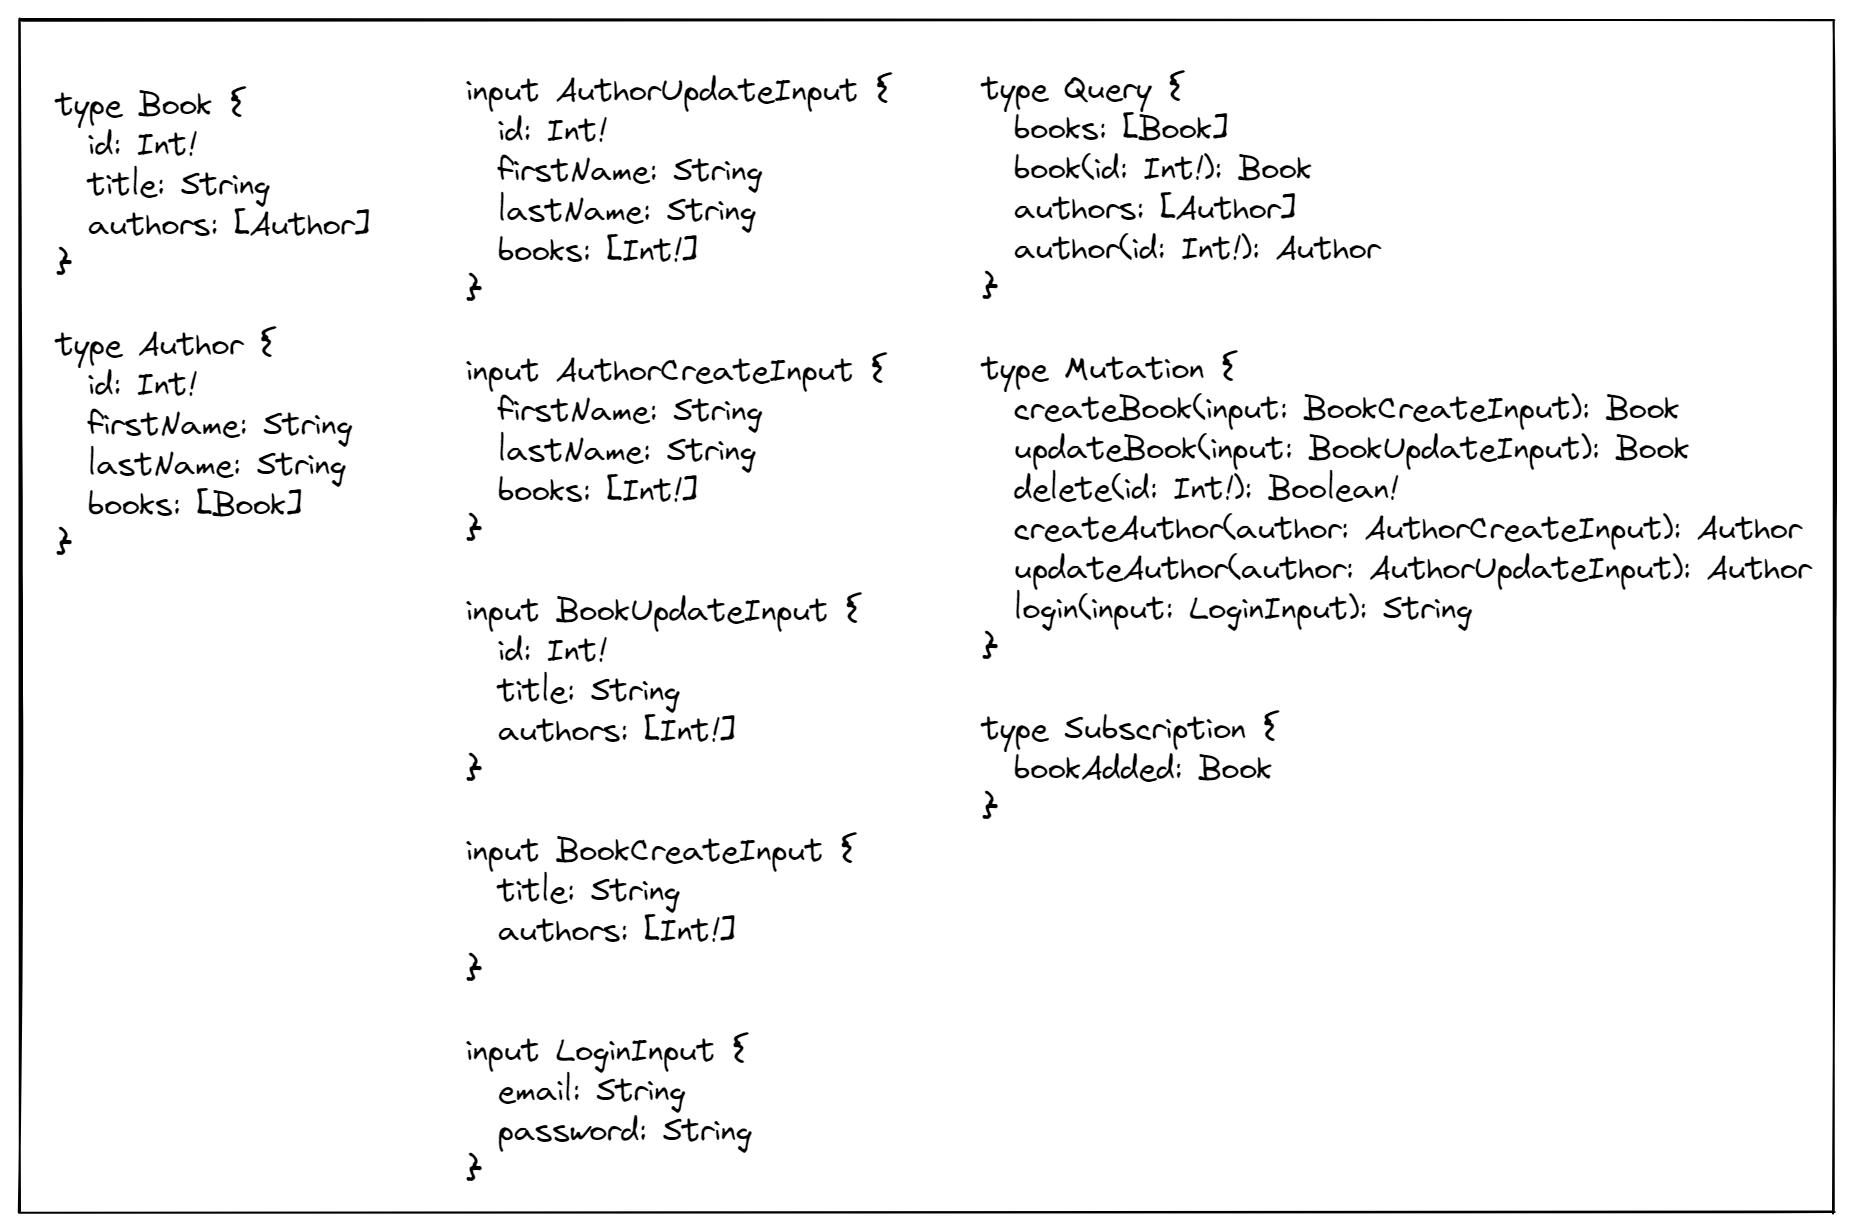
\includegraphics[width=\textwidth]{pics/schema.png}
%     \caption{Schemadefinition}
% \end{figure}

\begin{JsCode}
type Book {
    id: Int!
    title: String
    authors: [Author]
}
    
type Author {
    id: Int!
    firstName: String
    lastName: String
    books: [Book]
}
    
type Review {
    userId: Int!
    user: User!
    bookId: Int!
    book: Book!
    rating: Int!
    id: Int!
}
    
type User {
    firstName: String!
    lastName: String!
    email: String!
    roles: [Role!]!
    reviews: [Review!]!
    id: Int!
}
    
input AuthorUpdateInput {
    id: Int!
    firstName: String
    lastName: String
    books: [Int!]
}
    
input AuthorCreateInput {
    firstName: String
    lastName: String
    books: [Int!]
}
    
input BookUpdateInput {
    id: Int!
    title: String
    authors: [Int!]
}
    
input BookCreateInput {
    title: String
    authors: [Int!]
}
    
input LoginInput {
    email: String
    password: String
}
    
input ReviewUpdateInput {
    id: Int!
    userId: Int!
    bookId: Int!
    rating: Int!
}
    
input ReviewCreateInput {
    userId: Int!
    bookId: Int!
    rating: Int!
}
    
input LoginDataInput {
    email: String!
    password: String!
}
    
input UserInput {
    firstName: String!
    lastName: String!
    email: String!
    password: String!
    id: Int!
}
    
type Query {
    books(where: BookFilterInput, order: [BookSortInput!]): [Book!]!
    book(where: BookFilterInput, order: [BookSortInput!]): Book
    authors(where: AuthorFilterInput, order: [AuthorSortInput!]): [Author!]!
    author(where: AuthorFilterInput, order: [AuthorSortInput!]): Author
    reviews(where: ReviewFilterInput, order: [ReviewSortInput!]): [Review!]!
    author(where: ReviewFilterInput, order: [ReviewSortInput!]): Review
}
    
type Mutation {
    register(input: UserInput): User
    login(input: LoginDataInput): String
    createBook(input: BookCreateInput!): Book!
    updateBook(input: BookUpdateInput!): Book!
    createAuthor(input: AuthorCreateInput!): Author!
    updateAuthor(input: AuthorUpdateInput!): Author!
    createReview(input: ReviewCreateInput!): Review!
    updateReview(input: ReviewUpdateInput!): Review!
}
    
type Subscription {
    bookAdded: Book
}
\end{JsCode}

In Abbildung 3.1 ist eine Schemadefinition zu sehen welche Objekt-Typen, Input-Typen und die Wurzeloperationen beinhaltet.

\subsection{Parameter}
Felder können zusätzlich noch Parameter halten.
Diese Parameter können den Rückgabewert des Feldes ändern um, das Feld noch flexibler zu machen.
\newline

\begin{JsCode}
enum Currency {
    EUR
    USD
    GBP
}

type Book {
    id: Int!
    title: String
    authors: [Author]
    price: (unit: Currency = EUR): Float
}
\end{JsCode}

Im oben angeführten Code-Beispiel wurde der Objekt-Typ \textit{Book} um ein Feld \textit{price} erweitert.
Bei einer Query auf das Feld \textit{price} des Objekts \textit{Book} kann ein Argument \textit{unit} mitgegeben werden um den tatsächlichen Verkaufswert in der richtigen Währung zu bestimmen.
Dabei wurde ebenfalls ein Standardwert definiert um \textit{unit} nicht zwingend als Parameter übergeben zu müssen.
\cite[S.62]{kress2020graphql}


\subsection{Variablen}
Mit Parametern ist es möglich zusätzliche Daten für spezielle Operationen an den GraphQL-Service zu schicken.
Diese können aber nur statisch in die Query eingetragen werden.
Deswegen kann eine GraphQL Operation zudem mit Variablen erweitert werden.
Dadurch hat man verstärkt die Möglichkeit Funktionen wiederzuverwenden.
Variablen müssen am Anfang einer Operation definiert werden und befinden sich während der Ausführung im Lebensraum der Operation.
Diese Variablen werden unter anderem für die Filterung der angeforderten Objekte verwendet.
\cite[Abs. 5.8]{graphqlOnline}
\newline

In der folgenden Abbildung ist eine Anfrage zu sehen welche das Buch mit der \textit{id = 1} anfordert. Dabei wird die id als Variable übergeben.

\begin{figure}[H]
    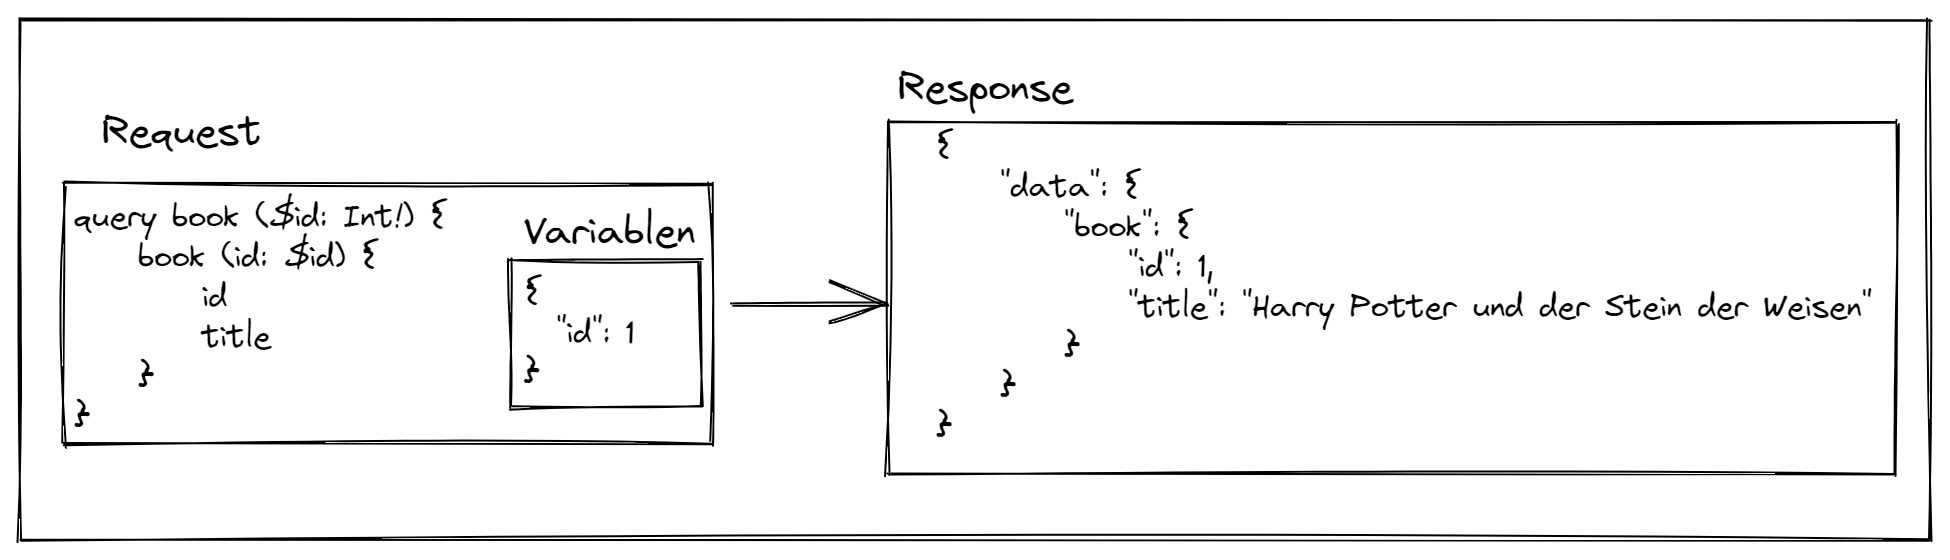
\includegraphics[width=\textwidth]{pics/book_request_with_parameter.png}
    \caption{Anfrage aller Bücher mit zugehörigen Autoren unter Verwendung einer Variable.}
\end{figure}

\section{Zugriff auf den GraphQL-Service}
GraphQL liefert keine Spezifikation der Netzwerkschicht, sondern lediglich eine Empfehlung, \textit{HTTP} zu verwenden.
Im Gegensatz zu \textit{REST-APIs} beschränkt sich GraphQL auf lediglich zwei HTTP-Methoden: GET und POST.
Deswegen ist die Gestaltung und Bennung der Endpunkte nicht so relevant wie bei REST-APIs.
\newline

GET und POST-Anfrage unterscheiden sich darin, dass mittels GET-Anfrage nur lesende Zugriffe möglich sind.
Also können mit GET-Anfragen nur Querys aber keine Mutations umgesetzt werden.
Desweiteren müsste man jede Query, als URL-Parameter übergeben.
Somit gilt es auch zu beachten die Sonderzeichen der Query in \textit{ASCII} umzuwandeln.
\newline

Wenn man nun also mittels GET-Anfrage eine Query an den GraphQL-Service schickt, resultiert es in dem Nachteil, dass man eine wesentlich schlechtere Übersicht hat. 
Denn die URL-Encodierung verkompliziert die Anfrage und sorgt für Einschränkungen in der Lesbarkeit.
Etwaig benötigte Variablen müssten auf dieselbe Art und Weise der Anfrage hinzugefügt werden.
Problematischer ist dabei aber jedoch, dass einige Browser eine Maximallänge für URIs vorgeben.
Somit können komplexe Querys nicht funktional sicher über GET-Anfragen abgebildet werden.
\newline

Aus diesem Grund werden üblicherweise alle Operationen auf POST-Anfragen abgebildet.
Diese werden an den einzigen, nach außen freigegebenen Endpunkt gerichtet.
Da für die Anfragen die POST-Methode verwendet wird, können im Body beliebig viele und komplexe Queries an den Service übergeben werden.
\newline

Grundsätzlich besteht eine Anfrage an den GraphQL-Service aus der eigentlichen Query und zwei optionalen Parametern: Variablen und der Name der Operation.


% Um schreibend oder lesend auf den GraphQL-Service zugreifen zu können muss an den bereitgestellten Endpunkt eine POST-Anfrage mit einer Query geschickt werden.
% Diese Query ist mittels der \textit{GraphQL Query Language GQL} definiert.
% Eine Anfrage welche eine Query beinhaltet, hat zusätzlich noch zwei optionale Parameter: \textit{variables} und \textit{operationName}.
% Der Name einer Operation wird jedoch nur benötigt wenn mehrere Operationen in der Query auszuführen sind.
% graphql.org/learn/serving-over-http

% Gress Seite 82-83

\section{Querys}

Querys bieten den Clients die Möglichkeit lesend auf die Objekte, welche vom GraphQL-Service verwaltet werden, zuzugreifen.
GraphQL erlaubt es dem Client genau die Daten abzufragen welche er benötigt.
Um auf eine Ressource zuzugreifen wird ein POST-Request an den Wurzelknoten der GraphQL-Applikation geschickt.
Dieser POST-Request enthält ein in der \textit{GraphQL Query Language} definiertes Objekt.
In diesem Objekt werden die auszuführenden Funktionen definiert und welche Felder davon an den Client zu retournieren sind.
Das Ergebnis hat genau jenes Format welches in der Anfrage vom Client definiert wurde \cite[S.40-41]{kress2020graphql}.
\newline

Da GraphQL mit einem Graphenschema arbeitet, welche auf den Beziehungen der Knoten zueinander basiert, ist es möglich diese Relationen zu nutzen um Daten über mehrere Objekte hinweg zu sammeln.
\newline

\begin{figure}[H]
    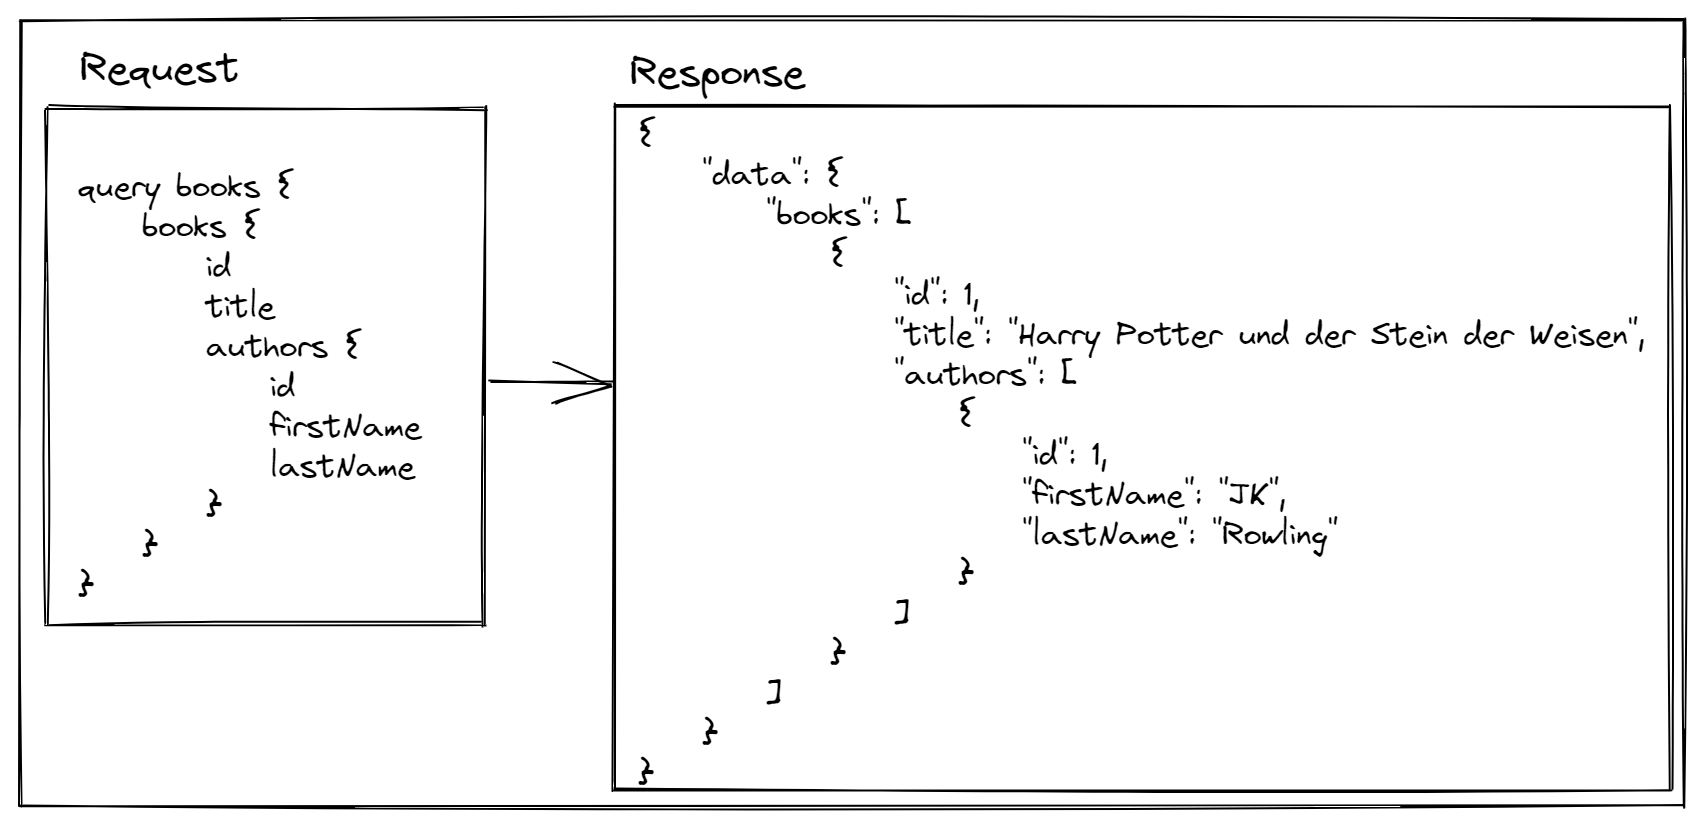
\includegraphics[width=\textwidth]{pics/query_book_with_result.png}
    \caption{Anfrage eines Buches mit ID=2.}
\end{figure}

Die in der obigen Abbildung ersichtliche Query fragt den Autor mit der ID=2 vom GraphQL-Service ab.
Dabei sollen die Bücher die der Autor geschrieben hat und mit dem Buch referenzierte Reviews ebenfalls zurückgegeben werden.
Um die in der obigen Abbildung angeführte Query ausführen zu können sind folgende Definitionen im Schema erforderlich:

\begin{JsCode}
type Author {
    firstName: String!
    lastName: String!
    books: [Book!]!
    id: Int!
}

type Book {
    title: String!
    authors: [Author!]!
    reviews: [Review!]!
    id: Int!
}

type Review {
    userId: Int!
    user: User!
    bookId: Int!
    book: Book!
    rating: Int!
    id: Int!
}

input AuthorFilterInput {
    and: [AuthorFilterInput!]
    or: [AuthorFilterInput!]
    firstName: StringOperationFilterInput
    lastName: StringOperationFilterInput
    books: ListFilterInputTypeOfBookFilterInput
    id: ComparableInt32OperationFilterInput
}

type Query {
    author(where: AuthorFilterInput): Author
}
\end{JsCode}

Aus dem Schema lassen sich folgende Entitäten herauslesen: \textit{Book}, \textit{Author} und \textit{Review}.
Weiters wurde ein \textit{AuthorFilterInput} deklariert, damit serverseitig nach einem bestimmten Buch sortieren werden kann.
Die Wurzeloperation Query enthält den Eintrittspunkt \textit{author}.
Dieser kann einen Filter entgegennehmen und liefert nach einer erfolgreichen Anfrage einen \textit{Author}, wobei dieser auch \textit{null} sein kann.

Die Anfrage die dem Server für das einholen der Daten geschickt wird enthält dabei folgenden Request-Body:

\begin{JsCode}
{
    "operationName": "author",
    "query": "query author($filter: AuthorFilterInput){
        authors(where: $filter){
            id
            lastName
            books {
                title
                reviews{
                    rating
                }
            }
        }
    }",
    "variables": {
        "filter": {
            "id": {
                "eq": 2
            }
        }
    }
}
\end{JsCode}

Der Request-Body ist dabei wie bereits erwähnt in 3 Teile unterteilt: \textit{operationName}, \textit{query}, \textit{variables}.
Diese Teile werden dann durch den GraphQL-Service zusammengefügt und nach erfolgreicher Validierung an die Resolver zur Evaluierung und Rückgabe der Daten weitergereicht.
Betrachtet man die Entitäten und ihre Referenzen als Baumstruktur, so ist bei der Evaluierung dieser Query der Autor die Wurzel, das Buch das Geäst und die Bewertung das Blatt des Baumes.
Die Resolver schreiten somit den Baum der angeforderten Entitäten bis zu den Blättern durch und geben dabei die angeforderten Daten an den Client zurück.

% \subsection{Aliase}
% In GraphQL-Queries ist es möglich, dass mehrere miteinander in Konflikt stehende Parameter übergeben werden.
% Um diesem Problem vorzuwirken besteht die Möglichkeit mit \textit{Aliases} zu arbeiten.
% Mit ihnen ist es möglich die unterschiedlichen Resultate dieser in Konflikt stehenden Argumente zu benennen und damit zu unterscheiden.
% % Kress 46
% \cite[S. 46]{kress2020graphql}

\section{Mutationen}
APIs benötigen neben dem lesenden Zugriff auf Daten auch einen schreibenden.
Dieser wird in GraphQL mittels Mutationen umgesetzt.
Mutationen kapseln die Implementierungen der Geschäftslogik in ein Interface welches die Möglichkeiten zur Manipulation der Daten vorgibt.
Manipulierende Anfragen können Daten dadurch nur auf jene Art und Weise ändern, wie es in der Applikation vorgesehen ist.
% Kress 54
\cite[S. 54]{kress2020graphql}

In der folgenden Abbildung ist eine Mutation zum hinzufügen einer Bewertung abgebildet:

\begin{figure}[H]
    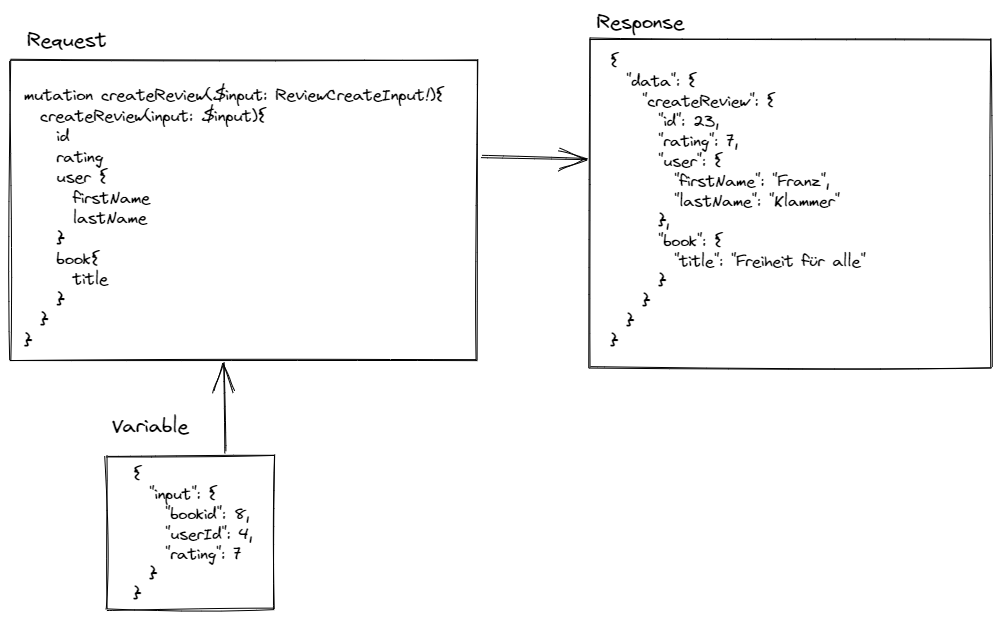
\includegraphics[width=\textwidth]{pics/createReviewMutation.png}
    \caption{Anfrage eines Buches mit ID=2.}
\end{figure}

Um eine Bewertung zu erstellen wird ein Input-Objekt \textit{ReviewCreateInput} und eine Mutation \textit{createReview} welches ein solches Objekt entgegennimmt benötigt.

\begin{JsCode}
input ReviewCreateInput {
    userId: Int!
    bookId: Int!
    rating: Int!
}

type mutation {
    createReview(input: ReviewCreateInput!): Review!
}
\end{JsCode}

\begin{JsCode}
{
    "operationName": "createReview",
    "query": "mutation createReview($input: ReviewCreateInput!){
        createReview(input: $input){
            id
            rating
            user {
                firstName
                lastName
            }
            book{
                title
            }
        }
    }",
    "variables": {
        "input": {
        "bookId": 8,
        "userId": 4,
        "rating": 7
        }
    }
}
\end{JsCode}

Der oben angegebene Request-Body der Anfrage ist wie bei der Query wieder in die drei Teile \textit{operationName}, \textit{query}, \textit{variables} aufgeteilt.
Diese werden wieder durch den GraphQL-Service an den verantwortlichen Resolver weitergeleitet.

\section{Subscriptions}
% Durch diese spezielle Form der Querys ist es möglich Daten in Echtzeit zu folgen und Updates direkt vom Server zu erhalten wenn gewisse Events ausgelöst wurden.
% Diese Events werden meist durch das Erzeugen, ändern oder löschen von Daten ausgelöst.

Subscriptions sind eine spezielle Form von Query.
Sie werden verwendet um den Client vom Server aus über Events zu notifizieren.
Notifizierungen werden in der Regel durch Hinzufügen, Ändern oder Löschen von Datenbankobjekten ausgelöst.
Subscriptions halten eine aktive Verbindung zwischen dem GraphQL-Service und dem Client offen.
Diese Verbindung wird meistens mit WebSockets umgesetzt.
Mit Subscriptions ist es zum Beispiel möglich den aktuellen Bestand von Produkten immer direkt am Client verfügbar zu haben.
Mit dieser Information kann auf der Client-Seite gewährleistet werden, dass ein Benutzer nur ein Produkt kaufen kann, welches noch verügbar ist.
\newline

\begin{figure}[H]
    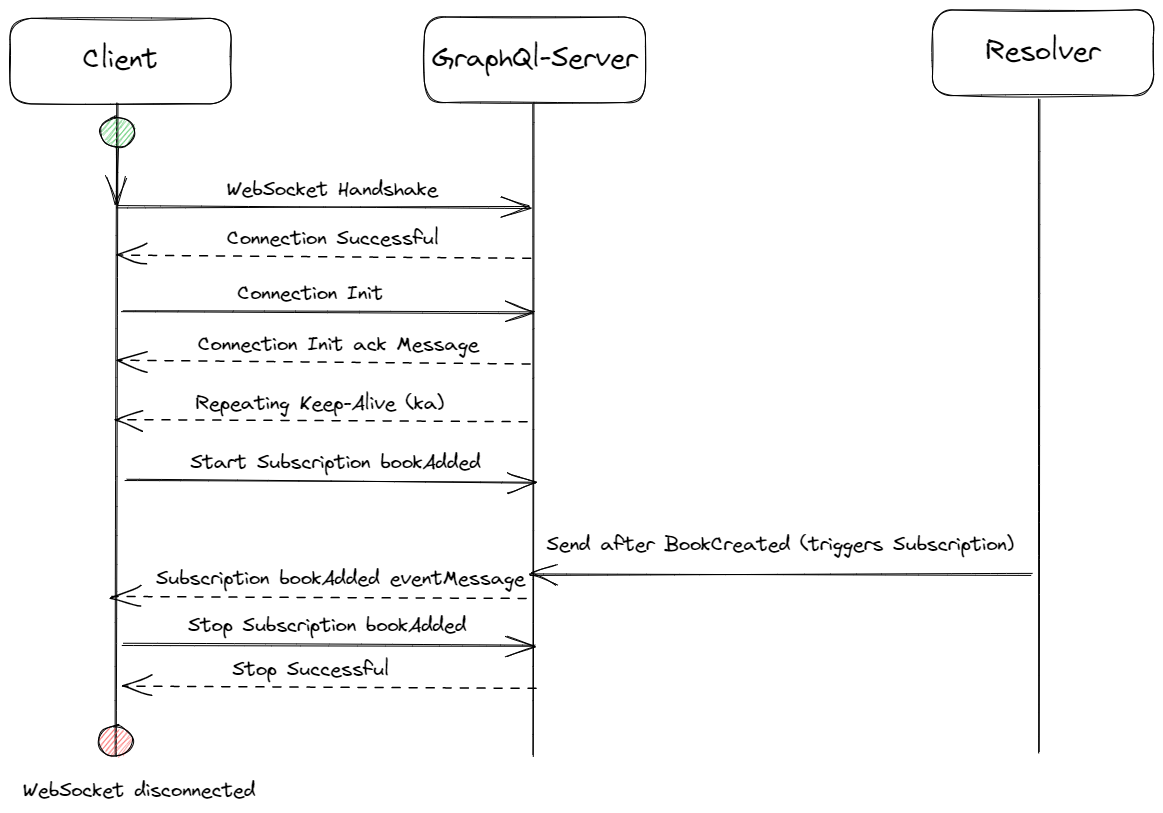
\includegraphics[width=\textwidth]{pics/SubscriptionWebSocket.png}
    \caption{Subscription die auf das Erstellen eines Buches wartet.}
\end{figure}

In der obigen Abbildung

Im folgenden Codebeispiel ist die Definition einer Subscription im Schema ersichtlich.

\begin{JsCode}
type Subscription {
    bookAdded: Book!
}
\end{JsCode}

% Weil sich der Server die Clients merken muss, ändert sich der Status des Systems von einem \textit{statless} zu einem \textit{stateful} API.
% Dadurch wird wiederum die Komplexität des Systems erhöht und die Skalierbarkeit erschwert.

\section{Bekannte Probleme}

